\begin{frame}
	\manimate
	\frametitle{Алгоритми}
	\begin{enumerate}
		\item Віднімання фону ( медіана, Гауса )
		\item Байесовський класифікатор
		\begin{enumerate} 
			\item Класична реалізація
			\item Поправки ймовірностей
			\item Удосконалений метод навчання
		\end{enumerate}
		\item Розпізнавання на основі сенсора глибини ( Intel Realsense F200 camera)
	\end{enumerate}
	
\end{frame}

\begin{frame}
	\manimate
	\frametitle{Віднімання фону}
	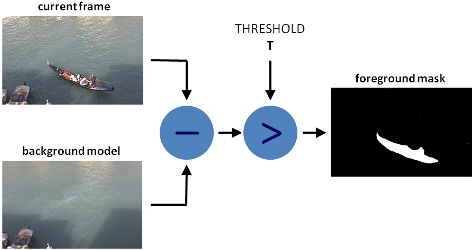
\includegraphics[width=1.0\linewidth]{im/background_substraction}
\end{frame}

\begin{frame}
	\manimate
	\frametitle{Байесовський класифікатор}
	\begin{equation}
		P(S|C) = \frac{P(C|S) * P(S)}{P(C)}
	\end{equation}
	подія $S$ - колір являється кольором людської руки \\
	подія $C$ - колір приймає значення $C$ \\
	де $\frac{P(S)}{P(C)}$ можна вважати деякою константою
\end{frame}

\begin{frame}
	\manimate
	\frametitle{Фільтрація ймовірностей байесовського класифікатора, сусіди}
	Цей підхід враховує лише факт нявності у деякої ймовірності сусідів у колі з радіусом $R$.
	\begin{enumerate}
		\item Підрахування кількості сусідів виконується згорткою з ядром у формі круга з радіусом $R$, заповненого одиницями.
		\item У матриці ймовірностей зануляються усі ймовірності, які мають менше сусідів ніж задане порогове значення.
	\end{enumerate}

\end{frame}

\begin{frame}
	\manimate
	\frametitle{Фільтрація ймовірностей байесовського класифікатора, зглажування}
	Цей підхід заснований на проведенні зглажування матриці ймовірностей та проводиться в 2 етапи:
	\begin{enumerate}
		\item Зглажування матриці ймовірностей $A$ за допомоги гаусівського ядра. $B = [b]_{ij}$ - результуюча матриця;
		\item $ (b{ij} < eps) => (a_{ij} = 0)$.
	\end{enumerate}
\end{frame}

\begin{frame}
	\manimate
	\frametitle{Фільтрація ймовірностей, до}
	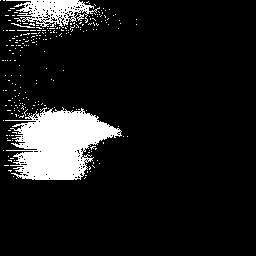
\includegraphics{b_start_gen}
\end{frame}

\begin{frame}
	\manimate
	\frametitle{Фільтрація ймовірностей, після}
	
\includegraphics{b_end_gen}
\end{frame}

\begin{frame}
	\manimate
	\frametitle{Відеопотік камери глибини}
	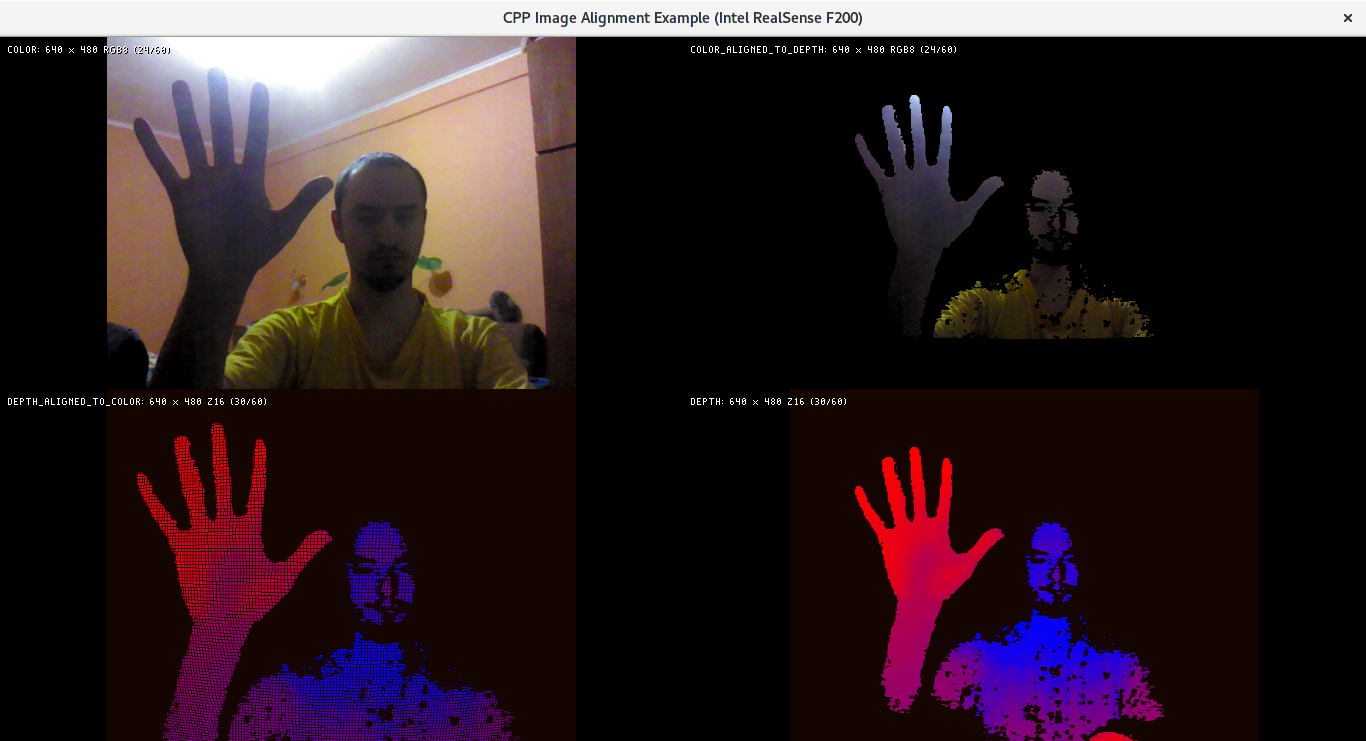
\includegraphics[width=1.0\linewidth]{im/depth_camera}
\end{frame}